\documentclass[11pt,a4paper,twoside]{book}

\usepackage{ngerman}
\usepackage{graphicx}
\usepackage{epsfig}
\usepackage{epstopdf}
\usepackage[onehalfspacing]{setspace}
\usepackage[hidelinks]{hyperref}
\usepackage{tocloft}
\usepackage{tikz}
\usepackage{float}
\usepackage{amsmath}

% Seitenlayout anpassen
\setlength{\textheight}{25cm}
\setlength{\textwidth}{17cm}
\setlength{\topmargin}{-15mm}
\setlength{\parindent}{0ex}
\setlength{\parskip}{2ex}
\setlength{\oddsidemargin}{-6.5mm}
\setlength{\evensidemargin}{-16.5mm}

% Inhaltsverzeichnis anpassen
\renewcommand{\cftchapfont}{\bfseries} % Kapitel fett
\renewcommand{\cftsecfont}{}           % Sektionen nicht fett
\renewcommand{\cftdotsep}{2}           % Punkte zwischen Titel und Seitenzahl

% Literaturverzeichnis alphabetisch und mit anderem Titel
\usepackage[backend=biber,style=numeric,sorting=nyt]{biblatex}
\addbibresource{Thesis_BIB.bib}
\AtBeginDocument{
  \renewcommand{\bibname}{Literaturverzeichnis}
}

\begin{document}

% Deckblatt und Verzeichnisse
\pagenumbering{roman}
%%%%%%%%%%%%%%%%%%%%%%%%%%%%%%%%%%%%%%%%%%%%
% deckblatt-BT-ET-IT-ger-v20170301.tex
% Deckblatt 
% Bachelorstudiengang Elektrotechnik
% Studienrichtung Elektrotechnik & Informationstechnik
%
% author:        		K.H. Hofmann 
% created:       	07.08.2014
% last revision:	01.03.2017
%%%%%%%%%%%%%%%%%%%%%%%%%%%%%%%%%%%%%%%%%%%%

% Page border should be:
% top: 15 mm
% oddside:  left 25 mm, right 15 mm
% evenside: left 15 mm, right 25 mm
%
% Eingaben
\newcommand{\Bearbeiter}{Moritz Mühlhausen}
\newcommand{\Thema}{Anomaliedetektion zur Entwicklung eines Predictive Maintenance Systems in der Verkehrstechnik}
%%%%%%%%%%%%%%%%%%%%%%%%%%%%%%%%%%%%%%%%%%%%
%\begin{document}
%%%%%%%%%%%%%%%%%%%%%%%%%%%%%%%%%%%%%%%%%%%%
% Deckblatt 1. Seite 
\thispagestyle{empty} 
%
\vspace{-20mm}
\begin{minipage}[t]{8cm}  

\epsfig{file=deckblatt/Logo-HsRm-1.eps,width=6cm}
\end{minipage}
\hfill
\raisebox{4.3ex}{\small \begin{tabular}[t]{l}
{\textbf{Fachbereich}} \\
Ingenieurwissenschaften \\[1ex]
{\textbf{Studienbereich}} \\
Informationstechnologie und Elektrotechnik \\[1ex]
{\textbf{Studiengang}} \\ 
Elektrotechnik \\[1ex]
{\textbf{Studienrichtung}} \\ 
Elektrotechnik \& Informationstechnik 
\end{tabular}}
\vspace{30mm}
\begin{center}{\Huge\bf Bachelor Thesis} \par
\vspace{20mm}
{\LARGE\bf  \Thema} \par
\vspace{16mm}
{\LARGE\bf  \Bearbeiter} \par
\end{center}
% 
\vspace{15mm}
\begin{flushright}
    Vorgelegt am (Stempel des Studienbereichs): \\
    \vspace{20mm} % Wenn mehr Platz nötig ist
    \rule[0ex]{\textwidth}{0.4pt} \hspace{5mm} (Ort / Datum) \hspace{30ex} (Unterschrift Student)
\end{flushright}
\vfill
\begin{flushleft}
\begin{tabular}{ll}
    Referent:	 &  Prof.\ Dr.-Ing. Michael Voigt \\ [0.5ex]
    Korreferent:	 &  M. Sc. Felix Becker, Vitronic Machine Vision GmbH
\end{tabular}
\end{flushleft}
%%%%%%%%%%%%%%%%%%%%%%%%%%%%%%%%%%%%%%%%%%%%
% Blankoseite
\newpage
\thispagestyle{empty}
\rule[0ex]{0ex}{0ex} 	% unsichtbare Markierung, damit Leerseite möglich
%%%%%%%%%%%%%%%%%%%%%%%%%%%%%%%%%%%%%%%%%%%%
% Versicherung
\newpage
\thispagestyle{empty} 
%
{\bf Versicherung}
\par
Hiermit versichere ich, dass ich die vorliegende Arbeit selbst\"andig und ohne unzul\"assige Hilfe Dritter verfasst 
habe.
\par
Die aus fremden Quellen direkt oder indirekt \"ubernommenen Texte, Gedankeng\"ange, Konzepte usw.\ in meinen 
Ausf\"uhrungen habe ich als solche eindeutig gekennzeichnet und mit vollst\"andigen Verweisen auf die jeweilige 
Urheberschaft und Quelle versehen.
\par
Alle weiteren Inhalte wie Textteile, Abbildungen, Tabellen etc.\ ohne entsprechende Verweise stammen im 
urheberrechtlichen Sinn von mir.
\par
Die vorliegende Arbeit wurde bisher weder im In- noch im Ausland in gleicher oder \"ahnlicher Form einer anderen 
Pr\"ufungsbeh\"orde vorgelegt.
\par
Mir ist bekannt, dass ein T\"auschungsversuch vorliegt, wenn sich eine der vorstehenden Versicherungen als 
unrichtig erweist.
\par
\vspace{25mm}
\rule[0ex]{\textwidth}{0.4pt}
(Ort / Datum)\hspace{30ex}	(Unterschrift Student)
%%%%%%%%%%%%%%%%%%%%%%%%%%%%%%%%%%%%%%%%%%%%
% Erklärung zur Einsicht in die Arbeit
\newpage
\thispagestyle{empty} 
%
Der Einsicht in die Bachelor Thesis  und der Ausleihe eines Exemplars der Thesis stimme ich zu / stimme ich nicht zu*.
\par\vspace{10mm}
\rule[0ex]{\textwidth}{0.4pt}
(Ort / Datum)\hspace{30ex}	(Unterschrift Studentin/Student)
\par\vspace{10mm}
Die Zustimmung kann nur bei Vorliegen eines berechtigten Interesses (z.B.\ laufende Forschungsprojekte / Patentschutz) 
verweigert werden. 
\par
Begr\"undung (bei Verweigerung): \\[5ex]
\rule[0ex]{\textwidth}{0.4pt} \\[2ex]
\rule[0ex]{\textwidth}{0.4pt} \\[2ex]
\rule[0ex]{\textwidth}{0.4pt} \\[2ex]
\rule[0ex]{\textwidth}{0.4pt} \\[2ex]
\rule[0ex]{\textwidth}{0.4pt} \\[5ex]
Nur vom Betreuer auszuf\"ullen: \\[2ex]
Gegen die Einsicht in die Bachelor Thesis  und gegen die Ausleihe eines Exemplars der Thesis wird / kein* Einspruch 
erhoben.
\par \vspace{10mm}
\rule[0ex]{\textwidth}{0.4pt}\\
(Ort / Datum)\hspace{30ex} (Unterschrift Betreuer)
\par
Begr\"undung (bei Einspruch): \\[5ex]
\rule[0ex]{\textwidth}{0.4pt} \\[2ex]
\rule[0ex]{\textwidth}{0.0pt} \\[2ex]
\rule[0ex]{\textwidth}{0.4pt} \\[2ex]
\rule[0ex]{\textwidth}{0.4pt} \\[5ex]
*Nichtzutreffendes bitte streichen
%%%%%%%%%%%%%%%%%%%%%%%%%%%%%%%%%%%%%%%%%%%%
%\end{document}
%%%%%%%%%%%%%%%%%%%%%%%%%%%%%%%%%%%%%%%%%%%%

\tableofcontents
\newpage
\listoffigures
\newpage
\listoftables
\newpage

% Wechsel zu arabischer Nummerierung, Kapitel
\pagenumbering{arabic}
\chapter{Einleitung und Motivation}
Vitronic Mautbrücken sind aufgrund ihrer schweren Erreichbarkeit und der Tatsache, dass sie über Autobahnen installiert
sind, eine besondere Herausforderung im Bereich der Wartung. Jede Inspektion oder Reparatur erfordert nicht nur die
Bereitstellung spezialisierter Techniker und Geräte, sondern auch eine präzise Planung, um Verkehrsstörungen zu
minimieren und die Sicherheit sowohl der Wartungsteams als auch der Verkehrsteilnehmer zu gewährleisten.

Ein technischer Defekt erfordert häufig eine komplexe Koordination mehrerer Teams und führt zu Verkehrsstörungen. Dadurch
entsteht die Notwendigkeit, Wartungseinsätze effizienter zu gestalten, um die Funktionalität der Infrastruktur und die
Sicherheit der Verkehrsteilnehmenden sowie der Servicemitarbeitenden zu gewährleisten. Gleichzeitig wächst der Druck, diese
Einsätze planbarer und seltener durchzuführen. Genau hier setzt die Motivation dieser Arbeit an: neue Methoden zu entwickeln, die
eine präzise Überwachung des Zustands der Brücken ermöglichen, ohne ständige physische Präsenz vor Ort.

Diese Arbeit befasst sich konkret mit der \textbf{Smart Sensor Platform X1}~-~kurz \textbf{SSPX1}, einem System zur
Erfassung, Verarbeitung und Weiterleitung von Bilddaten. Die vorhandenen Komponenten zur Mautüberwachung umfassen zwei Kameras,
ein eingebettetes High-Performance-Computermodul mit GPU-Unterstützung, ein High-Power-LED-Blitzmodul sowie
eine Stromversorgungshardware mit Weitbereichsspannungseingang. Die SSPX1 nutzt zahlreiche Sensordaten zur
kontinuierlichen und sorgfältigen Überwachung des Systemzustands.

\textbf{Predictive Maintenance} nutzt diese Daten, um Ausfälle vorherzusagen. Sie basiert auf der Analyse
von Echtzeitdaten, die aus einer Vielzahl von Sensoren entnommen werden können. Maschinelles Lernen bietet sich hier als effektive
Methode an, um sich anbahnende Fehler und Ausfälle vorherzusagen und abzufangen. So können Ressourcen effizient
genutzt und Ausfallzeiten minimiert werden~\cite{TobonMejia2012}.

Diese großen Datensätze werden über einen OPC UA Server zur Verfügung gestellt. OPC UA steht für \textit{Open Platform Communication
Unified Architecture} und ist ein Industriestandard für Datenaustausch sowie horizontale und vertikale Kommunikation, unter Anderem
aufgrund seiner Herstellerunabhängigkeit~\cite{Babel2024}.
Die Datenerfassung erfolgt lokal auf jeder SSPX1, welche im Zuge dessen auch einen eigenen Server betreibt, um die aufgenommenen
Daten bereitzustellen. Auf diese Weise wird eine dezentrale Sammlung relevanter Parameter wie Temperatur,
Leistung und Systemauslastung ermöglicht. Die kontinuierliche Überwachung und Speicherung dieser Daten in einer Datenbank
bildet die Grundlage für die Entwicklung und Anwendung prädiktiver Wartungsstrategien.

Ein zentraler Aspekt dabei ist die Detektion von Anomalien, die als Abweichungen vom normalen Verhalten definiert
werden~\cite{Chandola2009}. In multivariaten Systemen erschwert die hohe Dimensionalität und Komplexität der Daten ihre Erkennung.
Unüberwachte maschinelle Lernverfahren bzw.~\textbf{Unsupervised Learning} erweisen sich hier als besonders vielversprechend,
da sie Muster und Zusammenhänge in hochdimensionalen, unstrukturierten Datensätzen identifizieren können, ohne auf eine vorherige
Datenkennzeichnung angewiesen zu sein~\cite{Chandola2009, Wenig2024}.

Ziel dieser Arbeit ist es, Unsupervised Learning Algorithmen für die Erkennung und Interpretation von Anomalien in
heterogenen Datensätzen eines Systems in der Verkehrstechnik zu nutzen und damit die Effizienz von Predictive Maintenance
in der Verkehrstechnik zu optimieren. Dies soll durch eine frühzeitige Identifikation potenzieller Fehler erreicht werden.

Dabei wird zunächst in~\hyperref[ch:pdm_theorie]{Kap.~\ref*{ch:pdm_theorie}} ein theoretischer Hintergrund über die Grundlagen
von Predictive Maintenance und verschiedener Machine Learning Ansätze gegeben und warum sich Unsupervised Learning optimal für
die hier genannten Zwecke eignet.
% weitere Kapitel vorstellen ...

\newpage
\chapter{Zielsetzung}\label{ch:zielsetzung}
Eine effiziente Ressourcennutzung ist für Unternehmen von zentraler Bedeutung. Produktionsprobleme können dabei enorme finanzielle
Verluste verursachen, wie das Beispiel von Volkswagen im Jahr 2016 zeigt: Durch Störungen im Fertigungsprozess entstand ein wöchentlicher
Schaden von bis zu 400 Millionen Euro~\cite{Krupitzer2020}. Zudem zeigen Studien, dass je nach Branche zwischen 15 und 70~\% der
Produktionskosten auf wartungstechnische Ursachen zurückzuführen sind~\cite{Bevilacqua2000}.

Jedoch liegt der Fokus dieser Arbeit nicht auf wirtschaftlichen Faktoren. Trotzdem ist zu erwähnen, dass neue, effiziente
Wartungsstrategien basierend auf der Überwachung wichtiger Systemparameter insgesamt eine wirtschaftlichere und kostengünstigere
Alternative zu klassischen Wartungsstrategien (vgl.~\hyperref[sec:trad_maintenance]{Abs.~\Ref*{sec:trad_maintenance}})
darstellen~\cite{Deloux2009}~\Cite[S.~64--65]{Mobley2002}.

Der Fokus liegt vielmehr in der Entwicklung, Erprobung und Umsetzung der zugrundeliegenden technischen Fragestellung: \textbf{Wie können
Algorithmen zur Anomaliedetektion genutzt werden, um zur Entwicklung eines effizienten Wartungssystems
beizutragen?}

\begin{figure}[b!]
    \centering
    \begin{tikzpicture}
        \node[anchor=south west,inner sep=0] (image) at (0,0) {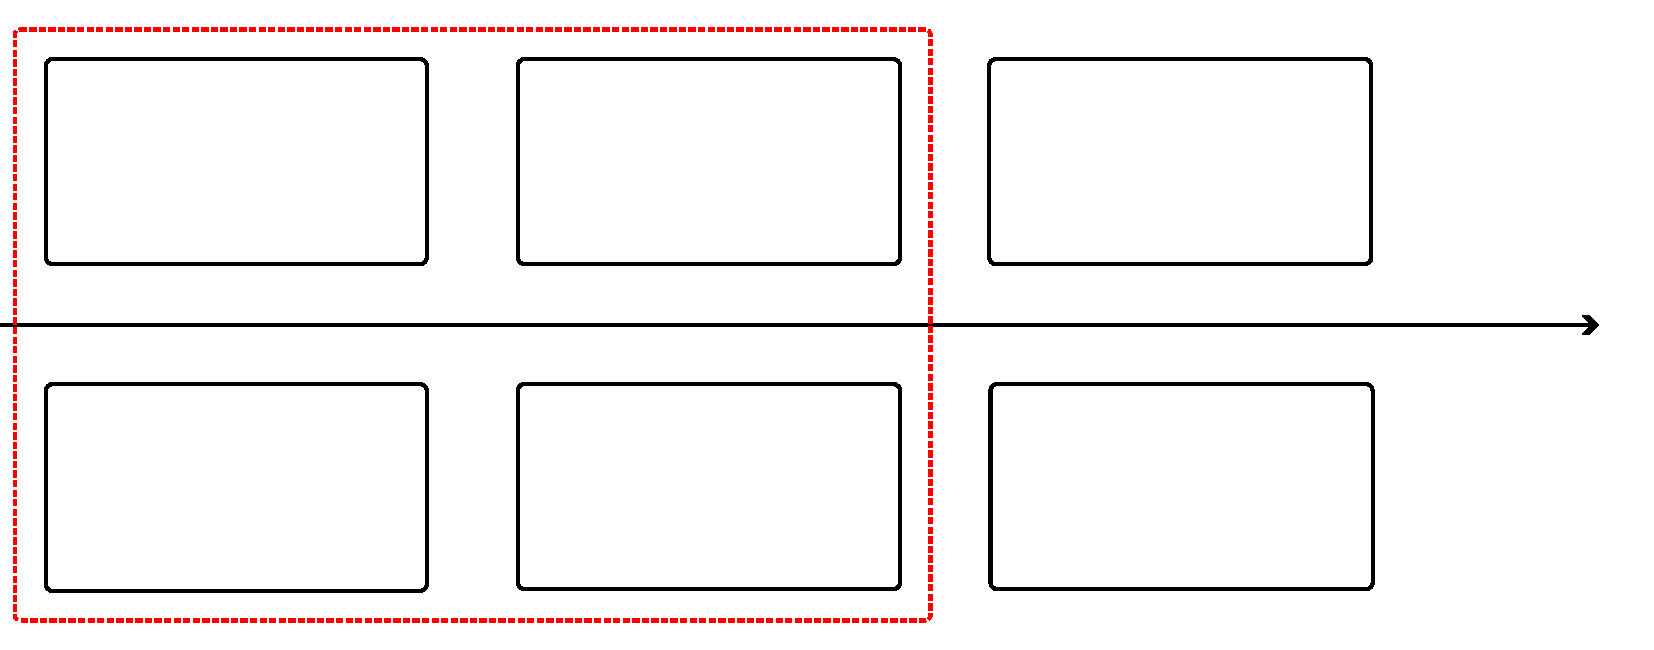
\includegraphics[width=1\linewidth]{ch2_zielsetzung/abbildungen/zielsetzung_scope.pdf}};
        % Koordinatensystem für die Grafik
        \begin{scope}[x={(image.south east)},y={(image.north west)}]
            % Textpositionen anpassen:
            \node at (0.145,0.74) {\large\parbox{6cm}{\centering Daten-\\aggregierung}};
            \node at (0.145,0.26) {\large\parbox{6cm}{\centering Recherche\\sich eignender\\Algorithmen}};
            \node at (0.43,0.74) {\large\parbox{4cm}{\centering Implementierung \&\\Erprobung der\\Algorithmen}};
            \node at (0.43,0.26) {\large\centering Evaluierung};
            \node at (0.715,0.74) {\large\parbox{4cm}{\centering Ableitung\\geeigneter\\Maßnahmen}};
            \node at (0.715,0.26) {\large\parbox{4cm}{\centering Schulen und Finden\\geeigneter\\Mitarbeiter}};
            \node at (0.85,0.46) {\centering Entwicklungsfortschritt};
            \node at (0.2875,0) {\centering \textcolor{red}{\large\textbf{Fokus der Arbeit}}};
            \node at (0.9,0.74) {\centering \dots};
            \node at (0.9,0.26) {\centering \dots};
        \end{scope}
    \end{tikzpicture}
    \caption{Entwicklungsprozess eines auf Predictive Maintenance basierenden Wartungssystems}
~\label{fig:zielsetzung_scope}
\end{figure}

Alle weiteren, impliziten Konsequenzen, wie eine Reduzierung der Downtime, Verbesserung der Systemzuverlässigkeit
und Gerätelaufzeit, eine Verbesserung der Produktqualität oder die Redundanz eines großen
Ersatzteillagers~\cite[S.~61--62]{Mobley2002}~\Cite[S.~5]{Scheffer2004} wollen im Rahmen dieser Arbeit nicht betrachtet werden.

Die starke Eingrenzung der Zielsetzung erfolgt auch aufgrund des gegebenen zeitlichen Rahmens der Arbeit von zehn Wochen. Das primäre
Ziel ist also vielmehr die Erprobung verschiedener, sich als potenziell geeignet heraustellender, Machine Learning Algorithmen zur
Anomaliedetektion. Dabei gibt es aufgrund der sich zum Teil sehr grundlegend unterscheidenden Arten von Anomalien entsprechend pro
Anomalietyp separate Kandidaten. Die voneinander abweichenden Anomaliearten und die dafür jeweils nominierten Algorithmen werden in
\hyperref[ch:anomalien]{Kap.~\Ref*{ch:anomalien}} vorgestellt und erläutert.

Die Erprobung der einzelnen Algorithmen erfolgt anhand der Anomalietypen, denen sie am besten zugeordnet werden können. Doch in
Studien zeigt sich, dass einzelne Algorithmen auch interdisziplinär, also für mehrere, sehr unterschiedliche Anomalietypen, gut
abschneiden~\cite[S.~30~-~31]{Wenig2024}\cite{Schmidl2022}. Daher sollen alle Algorithmen auch überschneidend getestet werden, um ein ganzheitliches Bild zu erhalten.
Der Kontext der Arbeit soll an dieser Stelle noch einmal hervorgehoben werden. Für industrielle Zwecke ist es vorteilhafter, sich auf eine
weniger umfangreiche Lösung zu konzentrieren, mit der aber mehrere Fehlerfälle abgedeckt oder vorhergesagt werden können, statt einzelne,
hochspezialisierte Lösungen zu finden. Die Robustheit eines Algorithmus ist daher genauso wichtig wie die Fähigkeit, jede Anomalie bis
ins letzte Detail zu erkennen. Auch diese Einordnung soll in der Findung der optimalen Lösung berücksichtigt werden.

Zur Bewertung und Einordnung der Ergebnisse der Algorithmen ist auch eine Evaluierungsmethode notwendig. Allerdings soll diese nicht
vollautomatisiert sein, sondern nach dem sog.~\textit{Human-in-the-Loop} Ansatz geschehen. So kann die Expertise geschulter und
erfahrener Mitarbeitenden in die Evaluierung miteingebunden werden, zur besseren Beurteilung und Korrektur der Ergebnisse~\cite{Deng2024}.

Schlussendlich und ausblickend soll diese Arbeit einen Beitrag zu besser getimten Wartungseinsätzen beitragen~-~nicht nur für die \ac{sspx1},
sondern für weitere Systeme der Vitronic Produktfamilie, da die zu Grunde liegenden, analysierten Parameter nicht exklusiv zur \ac{sspx1} gehören.
\newpage
\chapter{Wartungsstrategien}\label{ch:pdm_theorie}
Die zunehmende Komplexität und Vernetzung moderner Systeme erfordert effizientere Wartungsstrategien. Predictive Maintenance nutzt die
enormen Datenmengen solcher Systeme, um drohende Defekte frühzeitig zu erkennen und Ausfälle zu verhindern. Dadurch können
Ausfallzeiten minimiert und die Lebensdauer der Systeme verlängert werden.

Im Vergleich zu traditionellen Ansätzen bietet Predictive Maintenance signifikante Vorteile,
doch auch die klassischen Methoden haben ihre Berechtigungen. Diese werden im Folgenden diskutiert.

\section{Traditionelle Wartungsansätze}\label{sec:trad_maintenance}
Zu den traditionellen Wartungsansätzen gehören die reaktive und die präventive Wartung. Bei der reaktiven oder auch korrektiven
Wartung wird, gemäß der Namensgebung, erst bei vollständigem Ausfall von Komponenten gehandelt.
Der Vorteil dieser Methode liegt in der sehr geringen Planung und Überwachung. Für Komponenten,
die nicht kritisch oder essenziell sind, oder die ein sehr geringes Ausfallrisiko aufweisen, kann die reaktive Wartung sinnvoll sein.
Für alle anderen Bestandteile bzw.~die Gesamtheit eines Systems ist sie jedoch höchst ineffizient, da Wartungsmaßnahmen erst dann
veranlasst und geplant werden, wenn das System ausfällt. Zudem gestaltet sich die Diagnose dann auch als potenziell schwierig, da die
Fehlerquelle noch gefunden werden muss~\cite{Abdelli2022}.

Demgegenüber steht die präventive Wartung, die Maßnahmen am Ende eines vorher festgelegten Zeitintervalls oder nach Ablauf einer
bestimmten Betriebsdauer festlegt. Diese Zeitintervalle werden beispielsweise anhand der Badewannenkurve~\cite[S.~4]{Andrews2002},
wie in \hyperref[fig:bathtub]{Abb.~\Ref*{fig:bathtub}} dargestellt, auf Basis von Erfahrungswerten oder empirischen Untersuchungen geschätzt.
Die Badewannenkurve ist eine Darstellung der Ausfallverteilung, die die Wahrscheinlichkeitsverteilung von mechanischen oder elektrischen
Defekten beschreibt. Dieser Ansatz hat gewisse Vorteile für Komponenten, die nicht im dauerhaften Betrieb sind, sofern ausreichend geschultes Personal vorhanden
ist mit genügend Zeit, die Wartungsarbeiten durchzuführen. Nachteile liegen im potenziell schlechten Timing der Wartungsarbeiten, die
entweder zu früh oder zu spät stattfinden. Ohne Überwachung des Systemzustands ist schwer absehbar, in welchem Stadium seiner Lebensdauer
sich ein System befindet, und Komponenten, die noch eine gewisse Zeit weiterlaufen könnten, werden zu früh ausgetauscht. Durch die Wartung
verkürzt sich auch die Betriebsdauer des ganzen Systems und verursacht vermeidbare Kosten~\cite{Scheffer2004}.

\begin{figure}[H]
    \centering
    \begin{tikzpicture}
        \node[anchor=south west,inner sep=0] (image) at (0,0) {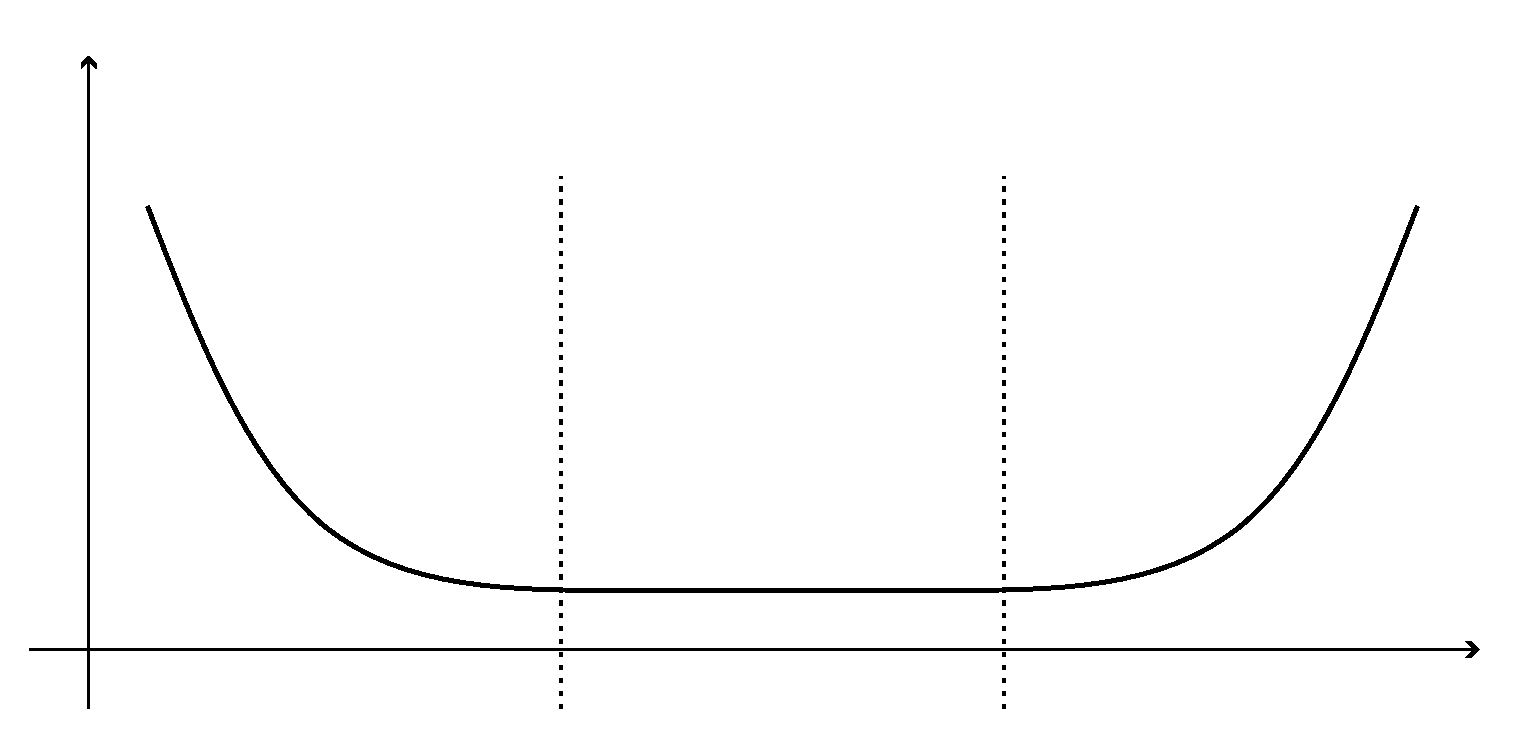
\includegraphics[width=\linewidth]{ch3_pdm_theorie/abbildungen/bathtub.pdf}};
        % Koordinatensystem für die Grafik
        \begin{scope}[x={(image.south east)},y={(image.north west)}]
            % Textpositionen anpassen:
            \node at (0.25,0.92) {\large\parbox{6cm}{Ausfallwahrscheinlichkeit}};
            \node at (0.88,0.05) {\large\centering Betriebsdauer};
            \node at (0.25,0.6) {\large\parbox{4cm}{\centering I\\Frühausfälle}};
            \node at (0.51,0.6) {\large\parbox{6cm}{\centering II\\normale Lebensdauer}};
            \node at (0.77,0.6) {\large\parbox{4cm}{\centering III\\Alterserscheinungen}};
        \end{scope}
    \end{tikzpicture}
    \caption{Badewannenkurve zur Visualisierung der Ausfallverteilung}
~\label{fig:bathtub}
\end{figure}

\section{Predictive Maintenance}
Nach Mobley~\Cite[S.~4]{Mobley2002} wird Predictive Maintenance als eine zustandsbasierte Wartungsstrategie definiert, die den
tatsächlichen Betriebszustand von Anlagen und Systemen überwacht, um Wartungsaktivitäten bedarfsgerecht zu planen.
Eine passende Analogie findet sich in der Medizin: Wenn der menschliche Körper Anzeichen einer bevorstehenden Krankheit zeigt, können
diese Symptome vom Arzt genutzt werden, um eine Diagnose zu stellen. Dementsprechend werden dann Maßnahmen ergeriffen, zum Beispiel
wird eine Behandlung eingeleitet oder Medikamente verordnet. Diese Zustandsüberwachung erlaubt es, dass Wartungsarbeiten zu einem
Zeitpunkt stattfinden können, der für alle Beteiligten passend ist und minimale Einschnitte in Produktions- oder Prozesslaufzeiten
bedeutet~\cite[S.~3]{Scheffer2004}.

Anhand von \hyperref[fig:pdm_workflow]{Abb.~\Ref*{fig:pdm_workflow}} ist zu erkennen, welche vereinfachten Schritte zur erfolgreichen
Implementierung eines Predictive Maintenance Systems erforderlich sind. Essentiell ist an erster Stelle eine adäquate Infrastruktur, die
sämtliche Zustandsparameter erfasst und gleichzeitig in der Lage ist, die erfassten Daten auch bereitzustellen. Es müssen im nächsten
Schritt Daten gesammelt werden, damit die im normalen Betriebszustand gültigen Schwellwerte ermittelt und festgelegt werden können.
Anhand dieser wird dann im laufenden, mittlerweile aufgenommenen Betrieb festgestellt, ob Abweichungen von den Parametern im Normalbetrieb
vorliegen. Demnach werden notwendige Wartungsarbeiten geplant und vorbereitet, wonach der Betrieb wieder ordnungsgemäß aufgenommen werden
kann.

\begin{figure}[H]
    \centering
    \begin{tikzpicture}
        \node[anchor=south west,inner sep=0] (image) at (0,0) {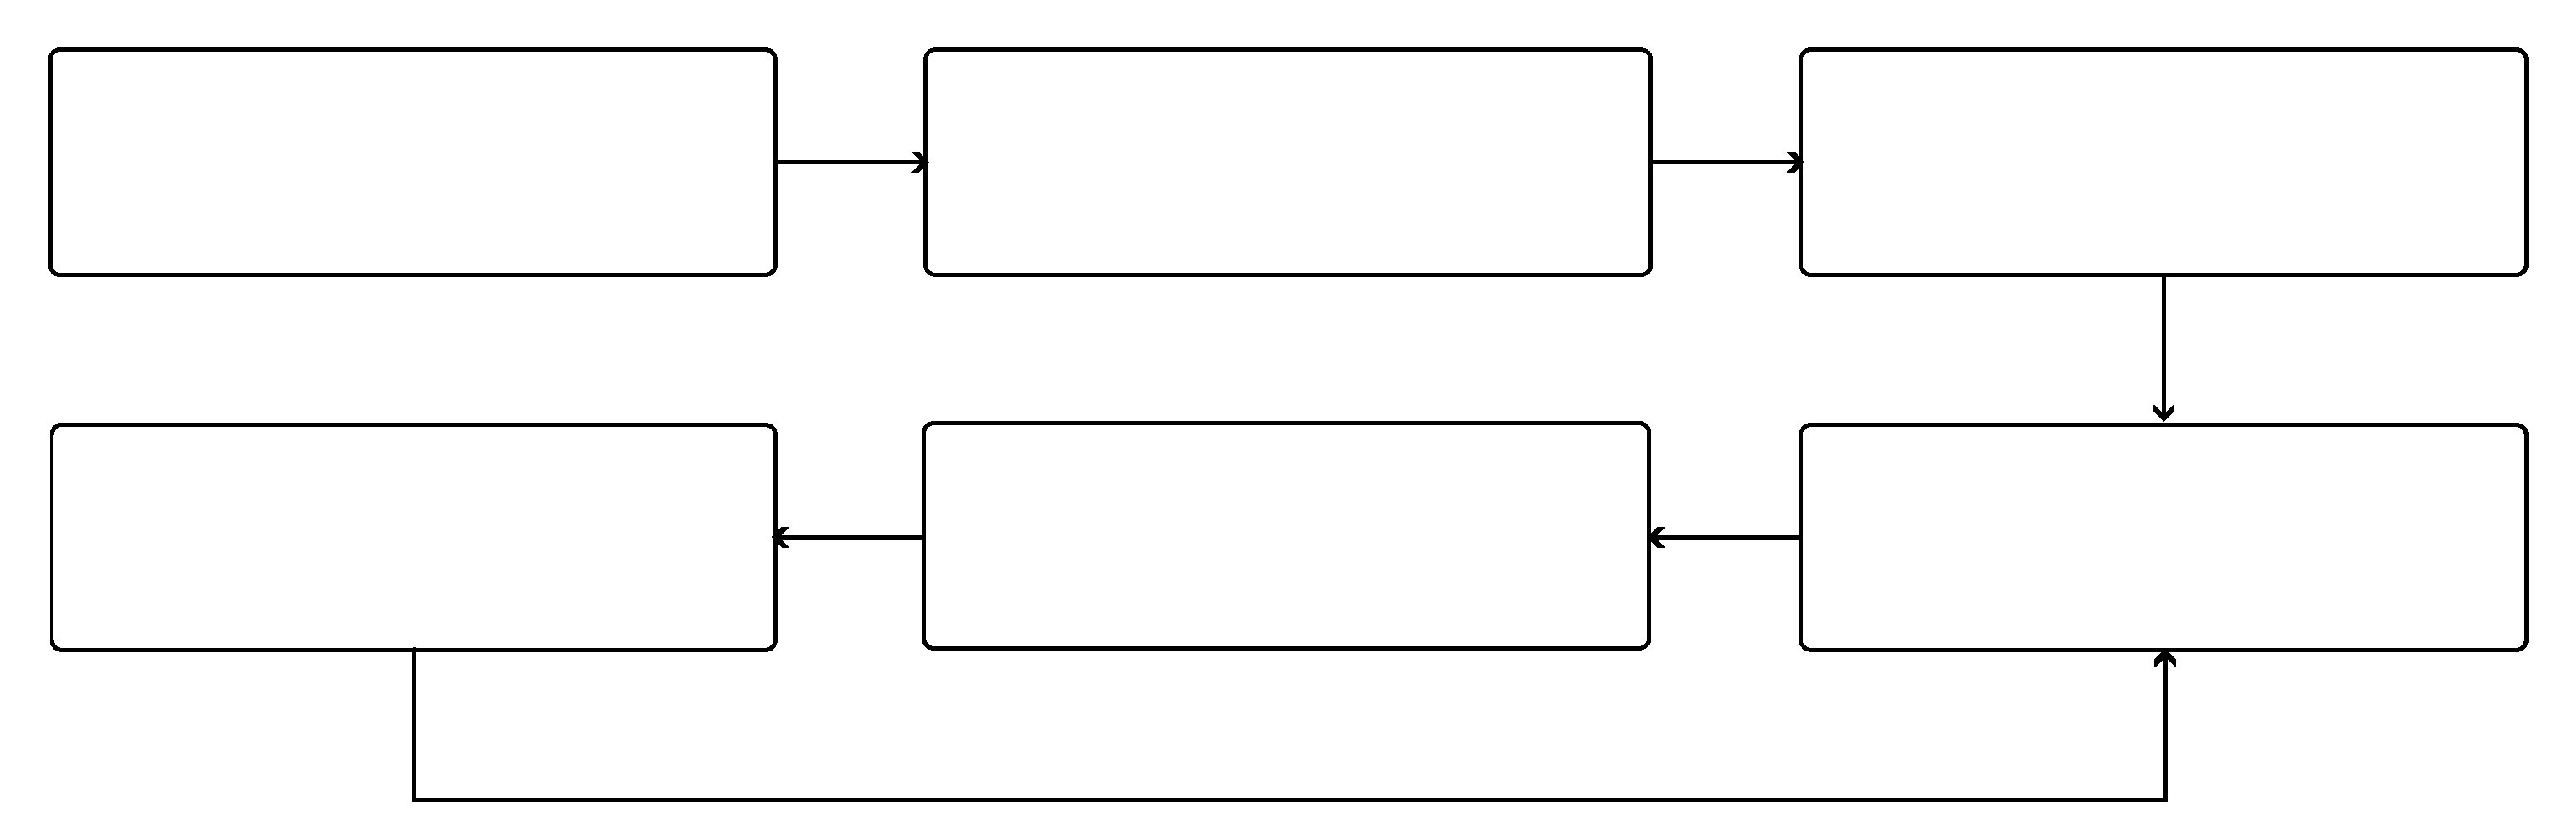
\includegraphics[width=\linewidth]{ch3_pdm_theorie/abbildungen/pdm_workflow.pdf}};
        % Koordinatensystem für die Grafik
        \begin{scope}[x={(image.south east)},y={(image.north west)}]
            % Textpositionen anpassen:
            \node at (0.16,0.815) {\large\parbox{6cm}{\centering Zustandsüberwachung\\einrichten}};
            \node at (0.5,0.815) {\large\parbox{6cm}{\centering Daten aggregieren}};
            \node at (0.84,0.815) {\large\parbox{6cm}{\centering Schwellwerte festlegen \&\\Parameter setzen}};
            \node at (0.84,0.35) {\large\parbox{6cm}{\centering normale\\Betriebsaufnahme}};
            \node at (0.5,0.35) {\large\parbox{6cm}{\centering Anomalien im\\Betrieb feststellen}};
            \node at (0.16,0.35) {\large\parbox{6cm}{\centering Wartungsarbeiten\\durchführen}};
        \end{scope}
    \end{tikzpicture}
    \caption{Workflow eines Predictive Maintenance Systems}
~\label{fig:pdm_workflow}
\end{figure}

Es stellt sich die Frage, welcher Anwendungsfall hauptsächlich interessant ist. In~\hyperref[ch:zielsetzung]{Kap.~\Ref*{ch:zielsetzung}}
wird bereits erläutert, in welchem Umfang eine Diagnose bzw.~Prognose gestellt werden soll. Vorrangig ist die Detektion von anomalem
Verhalten im laufenden Betrieb wie z.~B.~auftretende Alterserscheinungen oder Komponentenausfälle. Anhand dieser Anomalien soll durch
zusätzlichen menschlichen Input entschieden werden, ob und wann ein Wartungseinsatz notwendig ist.

Predictive Maintenance ist keineswegs eine neue Erscheinung. Der Ansatz und erste Methoden zur Umsetzung bestehen bereits seit den 70er
und 80er Jahren~\cite{Sandtorv1973, Renwick1985} mit Techniken wie beispielsweise der Vibrationsanalyse zur Zustandsbestimmung. Dabei
entwickelte sich der Fokus von Predictive Maintenance von lediglich der anfänglichen Überwachung durch die immer größer werdenden
Datenmengen hin zur ganzheitlichen Zustandsüberwachung. Durch technologische und industrielle Fortschritte wie Industrie 4.0 und dem
Internet of Things wurde die Umsetzung und Implementierung von Predictive Maintenance immer einfacher und kostengünstiger. Auf diese sog.
\textit{Enabling Technologies} wird in~\hyperref[sec:technologische_grundlagen]{Abs.~\Ref*{sec:technologische_grundlagen}} genauer
eingegangen.

Insgesamt zeigt sich das Konzept der Predictive Maintenance als natürliche Weiterentwicklung der traditionellen Wartungsansätze aufgrund
der einhergehenden technologischen Fortschritte. Während diese Arbeit lediglich Teilschritte zur Entwicklung eines Predictive Maintenance
Systems beitragen will, soll anhand der Erkenntnisse und Ergebnisse die Einführung und Nutzung eines solchen Systems die offensichtliche
Konsequenz sein.
\newpage
\chapter{Framework}\label{ch:framework}
Im Gegensatz zu diesen etablierten Methoden basiert Predictive Maintenance auf einem völlig anderen Ansatz, der auf kontinuierlicher
Überwachung und Datenanalyse beruht. In Anlehnung an Krupitzer et al.~\cite{Krupitzer2020} werden für die Entwicklung einer Predictive
Maintenance Lösung im Kontext des SSPX1 Mautüberwachungssystems einige Rahmenbedingungen skizziert. Diese lassen sich gem.
\hyperref[fig:pdm_framework]{Abb.~\Ref*{fig:pdm_framework}} kategorisieren.

\begin{figure}[H]
    \centering
    \begin{tikzpicture}
        \node[anchor=south west,inner sep=0] (image) at (0,0) {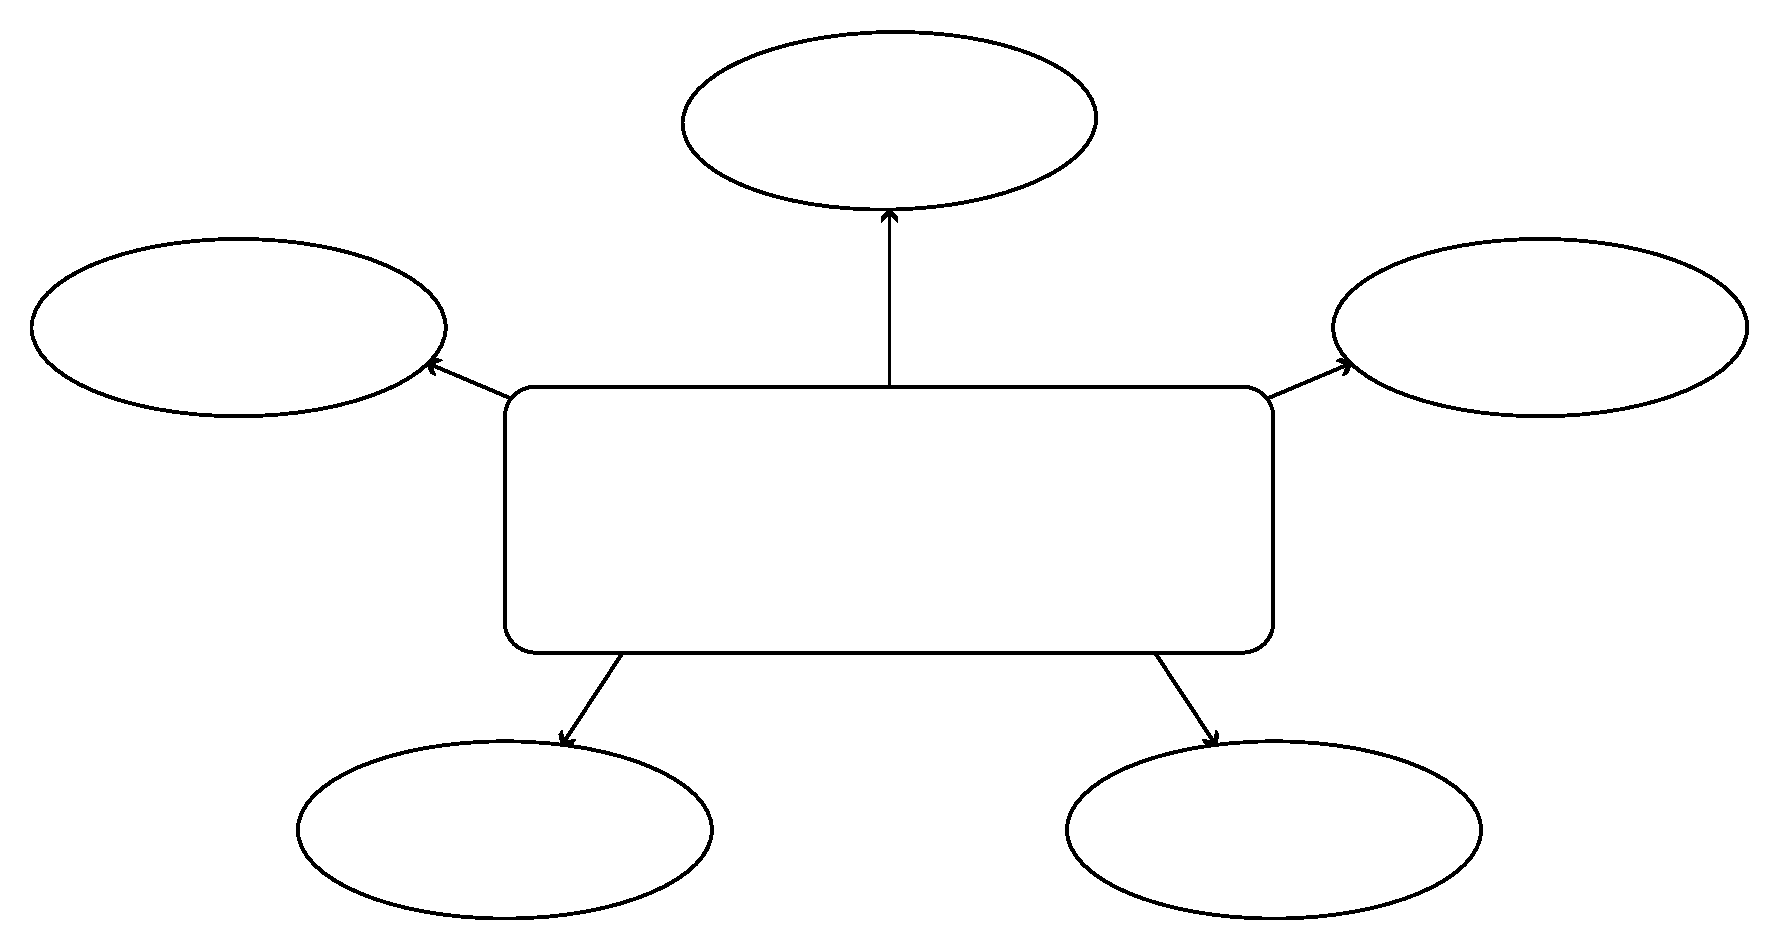
\includegraphics[width=\linewidth]{ch4_framework/abbildungen/framework.pdf}};
        % Koordinatensystem für die Grafik
        \begin{scope}[x={(image.south east)},y={(image.north west)}]
            % Textpositionen anpassen:
            \node at (0.5,0.45) {\Large\parbox{6cm}{\centering\textbf{Predictive Maintenance\\System Framework}}};
            \node at (0.13,0.65) {\large Evaluation};
            \node at (0.87,0.65) {\large \parbox{3cm}{\centering Technologische\\Grundlagen}};
            \node at (0.5,0.87) {\large Zielsetzung};
            \node at (0.28,0.13) {\large \parbox{3cm}{\centering Daten-\\verarbeitung}};
            \node at (0.72,0.13) {\large \parbox{3cm}{\centering Zustands-\\überwachung}};
            
        \end{scope}
    \end{tikzpicture}
    \caption{Framework zur Entwicklung eines Predictive Maintenance Systems}
~\label{fig:pdm_framework}
\end{figure}

\section{Technologische Grundlagen}\label{sec:technologische_grundlagen}
Die technologischen Grundlagen dieser Arbeit stützen sich auf die in der SSPX1 verbauten Sensoren, die präzise Systemdaten erfassen
und kontinuierlich überwachen. Zu den erfassten Parametern gehören unter anderem die Temperatur und Auslastung von GPU und CPU,
die Auslastung des Arbeitsspeichers sowie die Strom- und Leistungsaufnahme des Blitzermoduls.

Ein zentraler Baustein ist die Nutzung moderner IoT-Technologien in Kombination mit dem industriellen Kommunikationsstandard OPC UA.\
Dieser Standard ermöglicht einen effizienten und sicheren Zugriff auf die Sensordaten der SSPX1 und deren Übertragung an eine
Anwenderschnittstelle nach dem Client-Server-Prinzip~\cite{Babel2024}.

Da die Sensoren teilweise von unterschiedlichen Herstellern stammen und Messdaten in verschiedenen Formaten bereitstellen, sorgt OPC
UA für eine einheitliche und standardisierte Kommunikation. Die Daten werden dabei im kompakten \textit{OPC UA Binary}-Format~\cite{iec62541}
erfasst, wodurch eine performante und ressourcenschonende Datenübertragung ermöglicht wird. Anschließend werden die Daten an den OPC
UA-Server übermittelt und in der zugrundeliegenden SQL-Datenbank gespeichert. 

Durch diese Architektur wird eine herstellerübergreifende Interoperabilität gewährleistet, die OPC UA besonders für den betrachteten
Anwendungsfall geeignet macht. Die hohe Skalierbarkeit und Erweiterbarkeit des Standards ermöglicht zudem die einfache Integration
weiterer Sensoren und Systeme, wodurch zukünftige Erweiterungen ohne grundlegende Anpassungen der bestehenden Infrastruktur möglich
sind.

Ein weiterer Vorteil der Nutzung von OPC UA liegt in der serviceorientierten Architektur, die eine flexible Kommunikation
zwischen Client und Server ermöglicht. Der Client fungiert hierbei als Kommunikationsbrücke, die Anfragen und Antworten zwischen
der Anwenderschnittstelle und dem Server verwaltet. Die OPC UA-Kommunikations-Stacks unterstützen dabei die Datenverarbeitung und
gewährleisten eine robuste Übertragung, indem sie eng mit dem Speicher- und Dateisystem des Servers zusammenarbeiten. Zu den
wesentlichen Ereignissen der Client-Server-Kommunikation gehören~\cite{Babel2024,iec62541,Mao2024}:
\begin{itemize}
    \item \textbf{Message Requests:} Anfragen des Clients zur Datenabfrage oder -übertragung
    \item \textbf{Message Responses:} Antworten des Servers auf die Anfragen des Clients
    \item \textbf{Order Requests:} Aufrufe zur Ausführung bestimmter Serveraktionen
    \item \textbf{Notifications:} Benachrichtigungen über Änderungen oder Ereignisse im System
\end{itemize}

Darüber hinaus kann der OPC UA-Server als Bindeglied zwischen mehreren physischen Geräten oder auch als Cloud-Service fungieren,
was die Skalierbarkeit weiter erhöht und die Nutzung in verteilten Systemen erlaubt. Die Kombination aus präzisen Sensordaten,
standardisierter Kommunikation und einer skalierbaren Architektur bildet die technologische Grundlage für die Analyse und Umsetzung
von Predictive Maintenance im Rahmen dieser Arbeit.

\section{Zustandsüberwachung}\label{sec:zustandsueberwachung}
Ein wesentlicher Grund für ineffiziente Wartungsmaßnahmen liegt im unzureichenden Zugang zu Daten, die frühe Hinweise auf
potenzielle Schäden oder Ausfälle liefern könnten~\cite{Mobley2002}. Predictive Maintenance basiert auf der Voraussetzung, dass
Daten über den Zustand des betreffenden Systems oder der betreffenden Komponente zuverlässig verfügbar sind. Die Bereitstellung der
Daten erfolgt wie oben beschrieben mithilfe von OPC UA und die Zustandsüberwachung sensorbasiert.

Zu Beginn der Arbeit und in der Entwicklungsphase wird die Zustandsüberwachung einen inspektionsbasierten Ansatz verfolgen. Das
bedeutet, dass nach willkürlichen Intervallen immer auf die vom OPC UA Server zur Verfügung gestellten Daten zugegriffen wird und
diese Datensätze dann analysiert und weiterverarbeitet werden. Die Wahl dieser Methode basiert auf der geringeren Komplexität der
Implementierung in frühen Entwicklungsphasen und hat zur Folge, dass ein konsistenter Datensatz einen besseren Vergleich und
Feinabstimmung von Parametern der Analysetools ermöglicht.

Online Predictive Maintenance erweitert diesen Ansatz, indem sie eine kontinuierliche Überwachung des Systemzustands in Echtzeit
ermöglicht. Dabei werden Daten oder andere relevante Parameter in regelmäßigen Abständen automatisch erfasst. Nicht alle erfassten
Daten werden analysiert; vielmehr wird gezielt ausgewählt, welche Informationen für die Analyse und die Ableitung von Wartungsmaßnahmen
notwendig sind~\cite{Lindstroem2017}.

Die automatisierte Datenweiterverarbeitung als Teil der Online Predictive Maintenance erfolgt zu einem späteren Zeitpunkt und wird zu
Beginn noch nicht verfolgt, kann aber als schlussendliches Ziel gesetzt werden. So kann das in dieser Arbeit entwickelte System im
laufenden Betrieb optimal und effizient genutzt werden.

\newpage
\section{Datenverarbeitung}
Durch die kontinuierliche Aggregation von Messdaten der SSPX1 entstehen sehr große, hochdimensionale Datensätze. Jeder Datenpunkt in
der Zeitserie $S$ ist mehrdimensional. Formell lässt sich eine Zeitserie $S$ der Länge $n$ und Dimensionalität $d$ wie in
\hyperref[eq:timeseries_matrix_sum]{Gl. \Ref*{eq:timeseries_matrix_sum}a} definieren. $x_{i}^{j}$ ist der $i$-te Skalar der $j$-ten
Dimension einer Serie $S$. Für die Dimension $j={0,\dots,d}$ der Zeitserie $S$ entspricht jede Dimension einem Messwert im Datensatz. Da es
sich um eine Zeitserie handelt, entsprechen die Indizes $i={0, \dots, n}$ den Zeitstempeln der aufgenommenen Messwerte~\cite{Wenig2024}.

\begin{equation}
    \setcounter{equation}{0}
        \begin{subequations}
        \renewcommand{\arraystretch}{1.5}
        \begin{aligned}
            S &=
            \begin{bmatrix} 
                x_{0}^{0} & \cdots & x_{0}^{d} \\
                \vdots & \ddots & \vdots \\
                x_{n}^{0} & \cdots & x_{n}^{d} 
            \end{bmatrix} 
            && \text{(a)} \\[1.5em]
            S &= \sum_{i=0}^{n}\,\sum_{j=0}^{d}\,x_{i}^{j} \cdot E_{ij}
            && \text{(b)}
        \end{aligned}
    \end{subequations}
\label{eq:timeseries_matrix_sum}
\end{equation}


Alternativ kann die Zeitserie $S$ wie \hyperref[eq:timeseries_matrix_sum]{Gl. \Ref*{eq:timeseries_matrix_sum}b} in auch als Linearkombination
von Standardmatrizen geschrieben werden~\cite[S.~8]{Voigt2012}. Die elementweise Darstellung beschreibt die Matrix $S$ als Summe von
gewichteten Standardmatrizen $E_{ij}$, wobei jede Standardmatrix $E_{ij}$ genau an der Position $(i,j)$ den Wert 1 hat und sonst 0 ist.

% Literaturverzeichnis hinzufügen und verlinken
\addcontentsline{toc}{chapter}{Literaturverzeichnis}
\printbibliography[]

\end{document}
